\epigraph{Die Landkarte ist nicht das Territorium.}{Alfred Korzybski}

\section{Alles ist Eines --- aber welches Eine?}


\begin{figure}[htbp]
\centering
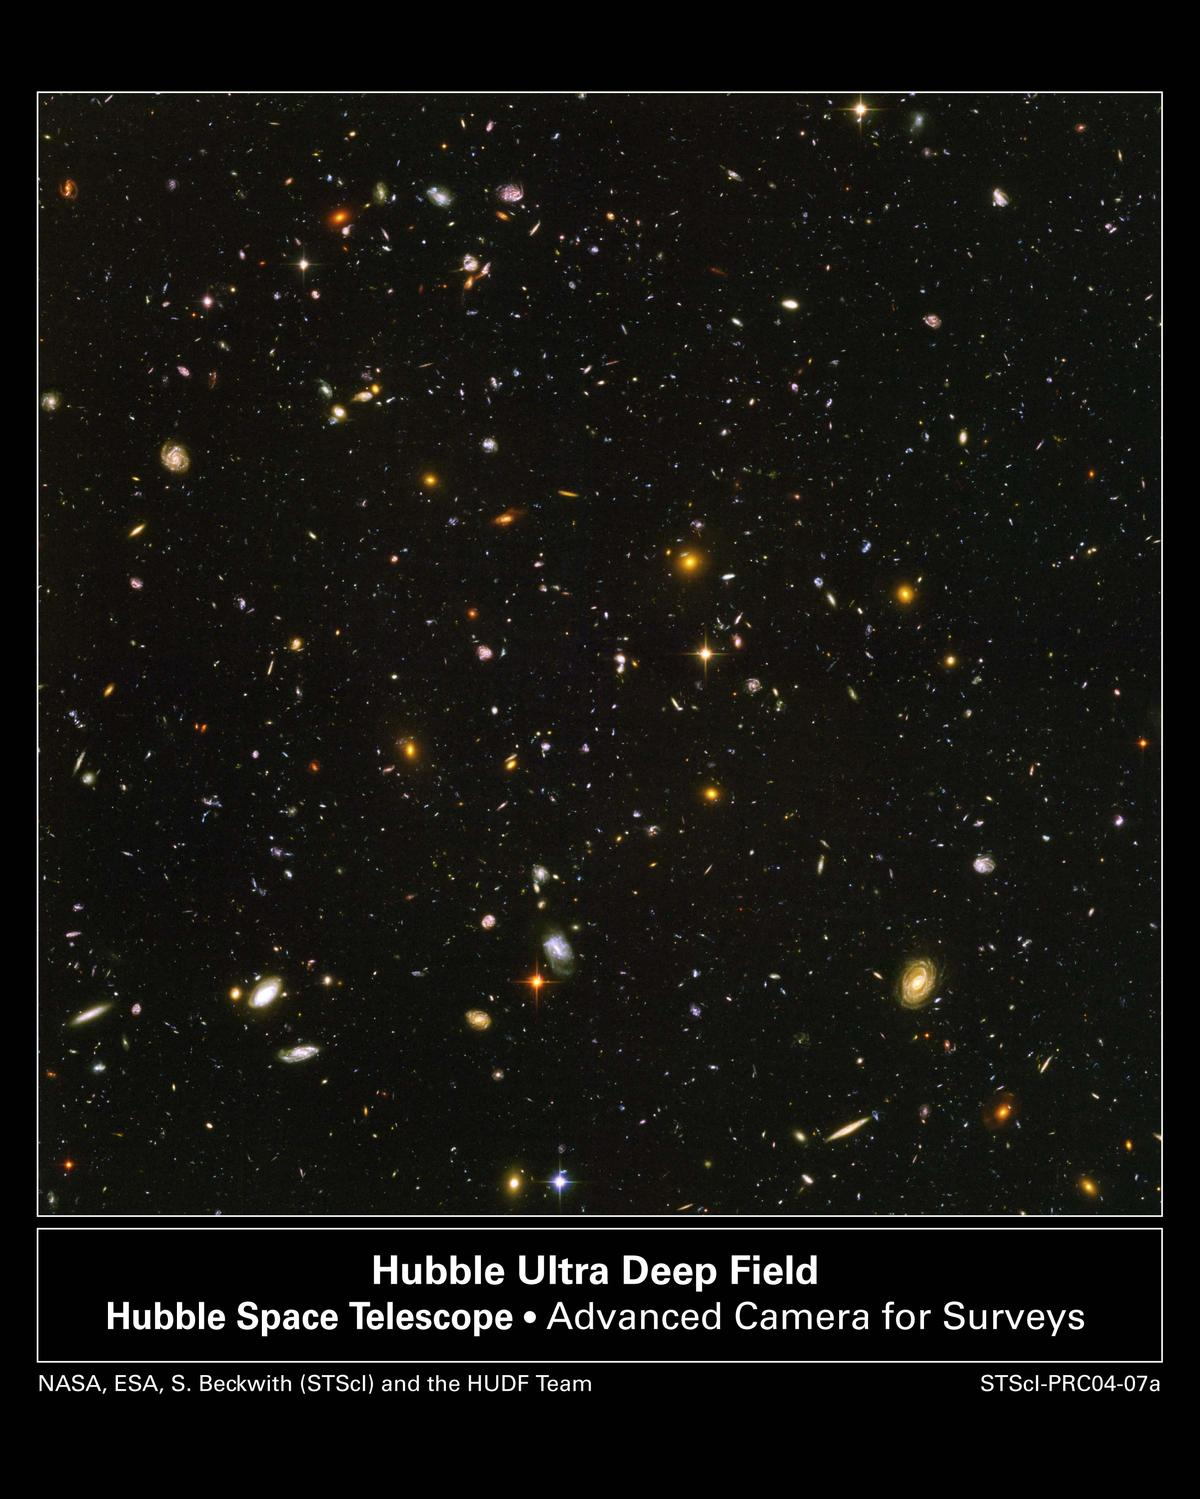
\includegraphics[width=0.85\textwidth]{img/hubble_udf_big.jpg}
\caption{Das Hubble Ultra Deep Field: Tausende Galaxien auf einem winzigen Himmelsausschnitt. In T0 entsteht Rotverschiebung durch Zeitfeldvariationen. Credit: NASA, ESA, S.~Beckwith (STScI), HUDF Team.}
\end{figure}
In T0 lässt sich alles auf eines der drei dualen Konzepte zurückführen: Alles ist Energie ($E$ als fundamentales Feld). Oder: Alles ist Masse ($m = E/c^2 = 1/T$). Oder: Alles ist Zeit ($T = 1/m$).

Die Wahl ist frei. Wählt man Energie als fundamental, existieren Masse und Zeit nicht als eigenständige Größen --- sie sind abgeleitete Schatten. Wählt man Zeit, werden Masse und Energie zu Frequenzen. Wählt man Masse, sind Zeit und Energie Kehrwerte und Produkte.

Es gibt kein \enquote{richtiges} Fundament. Die Dualität~$T \cdot m = 1$ sagt: Beide Seiten sind gleichberechtigt. Das Universum hat keinen privilegierten Beschreibungsmodus.

\section{Gott steht außerhalb des Systems}

Wenn das gesamte Universum ein Torus ist --- unendlich, begrenzt, singularitätsfrei ---, dann steht ein etwaiger Schöpfer \emph{außerhalb} dieses Systems. Nicht außerhalb der Zeit, denn Zeit ist nur eine Phasenkoordinate im Torus. Nicht außerhalb des Raums, denn Raum ist die Torusstruktur selbst. Sondern außerhalb des \emph{gesamten mathematischen Konstrukts}.

Die Theorie beschreibt das \emph{Wie} mit bemerkenswerter Präzision. Sie beschreibt nicht das \emph{Warum} --- warum es überhaupt etwas gibt statt nichts. Diese Frage liegt außerhalb der Reichweite jeder physikalischen Theorie, auch dieser.

\section{Unsere Konstrukte sind nicht die Realität}

Die Gleichungen --- $T \cdot m = 1$, $\Phi = \rho \cdot e^{i\theta}$, $\xsi = 4/30000$ --- sind \emph{Landkarten}, nicht das Territorium. Wir erfassen die Realität nie absolut.

Jedes Einheitensystem --- SI, natürlich, T0 --- ist eine Konvention. Jede Formel ist eine Approximation, selbst $\Kfrak = 0{,}9867$ ist eine Linearisierung. Die fraktale Dimension~$\Df \approx 2{,}9999$ ist eine Annäherung an etwas, das möglicherweise nicht einmal eine Zahl im üblichen Sinne ist.

Was die Theorie leistet: Sie zeigt, dass die Natur mit einem einzigen Parameter beschrieben werden kann --- eine atemberaubende Vereinfachung. Was sie nicht leistet: erklären, warum es überhaupt etwas gibt statt nichts.

Die Mathematik ist das mächtigste Werkzeug, das wir haben. Aber Werkzeuge sind nicht die Wirklichkeit selbst.

\begin{kerngedanke}
Je tiefer wir schauen, desto einfacher wird die Struktur --- aber die letzte Schicht bleibt uns verborgen. Vielleicht muss das so sein. Demut vor der Natur ist keine Schwäche einer Theorie, sondern ein Zeichen ihrer Reife.
\end{kerngedanke}
